\section{总体设计}

多功能计算器的主页面功能设计如\autoref{fig:Overall}所示。
\begin{figure}[!htbp]
    \centering
    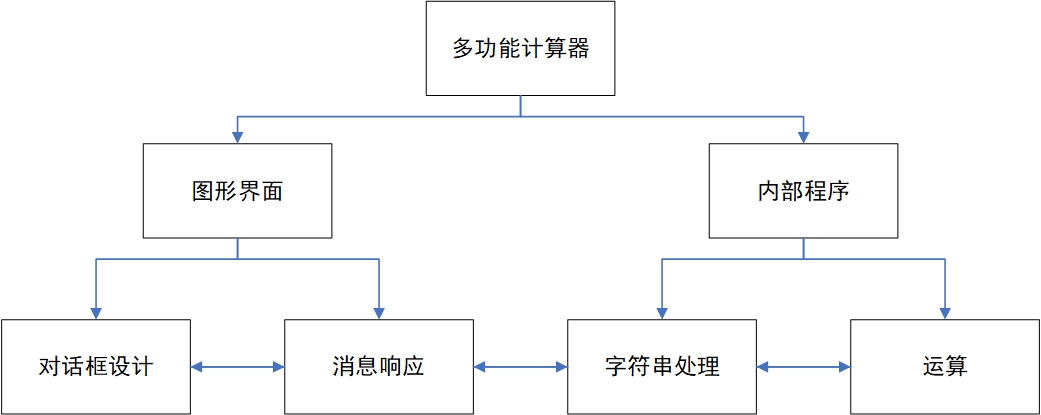
\includegraphics[width = 15cm]{总体设计图.jpg}
    \caption{总体设计图}
    \label{fig:Overall}
\end{figure}

其中,对话框、消息响应函数、字符串处理程序与运算程序均包含双向信息传递。在
单次运算中,用户通过图形界面输入算式,点击“=”后,算式字符串从编辑框被读取,
传递至字符串处理函数转化为数字与符号序列,再由运算程序计算结果;计算的结果返回
消息响应函数,实现对话框更新。

值得一提的是,本项目在菜单中增加了“描述性统计”和“矩阵运算”选项,这两个功能相对独立,
但仍然大致采用上图的信息处理流程。

\subsection{对话框}
如1.2节\autoref{fig:Advance},\autoref{fig:DesStat},\autoref{fig:MatrixManip}所示。


\subsection{消息处理函数}

对话框每一个控件都有单独的消息处理函数,根据功能可以分为三类,分别是:
\begin{enumerate}
    \item “=”的消息处理函数,负责获取编辑框算式,传递给字符串处理函数,并更新结果至编辑框;
    \item “高级”和“分数模式”的消息处理函数,负责管理对话框中按钮的显示与否,以及运算模式;
    \item 其余按钮的消息处理函数,负责输入算式。
\end{enumerate}

另外,还有菜单中选项的消息处理程序,其功能是创建对应的对话框。

\subsection{字符串处理程序与运算程序}
主界面的字符串处理与运算在逻辑上是两个分步过程,但实际中,我们利用栈实现了字符串解析与运算的并行化,
从而能很好地处理运算优先级。

“描述性统计”或“矩阵运算”的字符串处理和运算是分开进行的,比主界面更简单。

\subsection{难点}
本项目难点在于字符串解析和运算,因为有优先级和括号的存在,计算没有固定的顺序,所以必须实时解析并运算。